\documentclass[journal,11pt]{IEEEtran}
\usepackage{amsmath,amsfonts}
\usepackage{algorithmic}
\usepackage{array}
\usepackage[caption=false,font=normalsize,labelfont=sf,textfont=sf]{subfig}
\usepackage{textcomp}
\usepackage{stfloats}
\usepackage{url}
\usepackage{verbatim}
\usepackage{graphicx}
\usepackage{balance}

\hyphenation{op-tical net-works semi-conduc-tor IEEE-Xplore}
\def\BibTeX{{\rm B\kern-.05em{\sc i\kern-.025em b}\kern-.08em
    T\kern-.1667em\lower.7ex\hbox{E}\kern-.125emX}}

\begin{document}
\title{Parrellel Cuda Implementation of 3D DWT}
\author{Graham Pellegrini 0352804L}

\markboth{CCE3015 Assignment 2}{}

\maketitle

\begin{abstract}
    This report details the porting of a serial Multi-Level 3D Discrete Wavelet Transform (DWT) to a parallel implementation using CUDA. Key decisions, comparative approaches, and performance results are discussed, highlighting speedup and efficiency gains. The report concludes with an evaluation of results and future work directions for further optimization.
\end{abstract}
    

\section{Feedback Considerations}

The first assignment focused on the serial implementation of a Multi-Level 3D Discrete Wavelet Transform (DWT). For this assignment, the scope shifted to a single-level 3D DWT to emphasize parallelization using CUDA. Feedback from the previous assignment was incorporated to meet the requirements.\\

The report format, previously incorrect, has been updated to the IEEE Signal Processing template, with a double-column layout and minimum 11pt font size. Additionally, this report provides a more detailed analysis of testing and results, including the suggested inverse transform ('idwt.h') for comparison with the original image. Note the inverse image in figure 0 is lower quality due to the lossy nature of the DWT and a descrepancy of 1 in the depth occurs due to the dividing by 2 and rounding down and then multiplying by 2 again.\\

\begin{figure}[h]
    \centering
    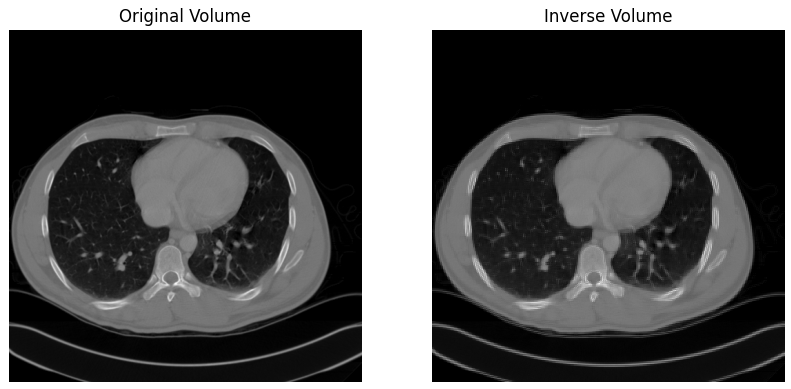
\includegraphics[width=0.5\textwidth]{assets/inverse.png}
    \caption{Original vs Inverse Image}
    \label{fig:1}
\end{figure}

Earlier plans proposed parallelizing all three dimensions of the 3D DWT simultaneously, but feedback noted that dependencies between dimensions made this infeasible. Instead, dimensions are processed sequentially, with separate kernels for each, and synchronization ensures one dimension's transform completes before the next begins. Contrary to earlier assumptions, no synchronization is needed within kernels, as thread indexing determines the section of the volume to process. Proper block and grid calculations ensure efficient thread management within the defined scope.\\

Kernel calls alternate input and output pointers to avoid extra memory management or data copying. Parallelizing I/O, as previously suggested, was not prioritized because CUDA kernels focus on computation, not data handling. As such, the existing I/O headers ('savebin.h' and 'loadbin.h') remain unchanged, with memory transfers handled by other CU functions.\\

In the kernel, on-the-fly vectors for sum low and sum high were initially substituted with shared memory caches, along with the coefficients, to potentially improve performance. However, after further evaluation, these were reverted to the constant memory implementation, as it was found to be more efficient in terms of memory access latency and overall kernel execution time.

\section{Project Structure}
The project meets all specified requirements for build configurations and naming conventions. The implementation is logically organized, with the main functionality and DWT implementation consolidated in 'assignment-2.cu' within the src folder to streamline the Makefile and avoid separate compilation complexities. Key includes are 'idwt.h' for inverse transform functionality, 'kernels.cuh' for individual 1D DWT and volume mapping kernels, and 'loadbin.h' and 'savebin.h' for binary file handling. The Makefile, located at the root is responsible for the project compilation.\\

The Makefile has been built to ensure support for the CUDA by using 'nvcc' and respective cuda includes are located within the files. Separate build configurations are provided for debug and release modes, where the debug build disables optimizations, enables assertions (-DDEBUG), and includes debug symbols (-g). Conversely, the release build optimizes for performance (-O2) while excluding debug symbols and assertions. Additionally, profiling support is incorporated through dedicated targets for NVIDIA tools (ncu and nsys). Which will enable the system profile analysis to identitfy regions of the code that can be further optimized or improvements made.

\section{Devision of Problem}

The main challenge that defines the structure for performing parallel operations is the fact that the volume must be treated as a whole. When performing dimension-wise DWT operations, the entire volume; containing all the rows, columns, and depth—must be considered to ensure the operations are executed correctly. This directly impacts how data management is handled and the order in which kernel operations and threaded access are managed.\\

Previously, the serial implementation consisted of a single 'dwt 1' function that handled the transformation along one dimension. However, in the parallel implementation, three separate kernels are defined, one for each dimension, to minimize excessive copying of temporary data. The 'dwt 3d' function defines a block with a dimension size of (16, 16, 4). Initially, other iterations and tests using sizes such as (256,1,1), (16,8,8) or (8, 8, 8). 

\begin{figure}[h]
    \centering
    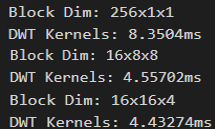
\includegraphics[width=0.3\textwidth]{assets/block-dims.png}
    \caption{Different Block Dimensions Tested}
    \label{fig:2}
\end{figure}
However, since our volume is more likely to have significantly larger dimensions in the rows and columns than in the depth, the depth (Z-dimension) was given a quarter of the block size. This ensures that the total threads in each block remains a factor 64 (16×16×4 = 1024). The choice of block size strikes a balance between generalization, by avoiding fine-tuning for one specific test volume case, and specification by addressing CT scans and 3D images whoes depth index will be at least four times smaller than the rows and columns constructing each slice.
\begin{figure}[h]
    \centering
    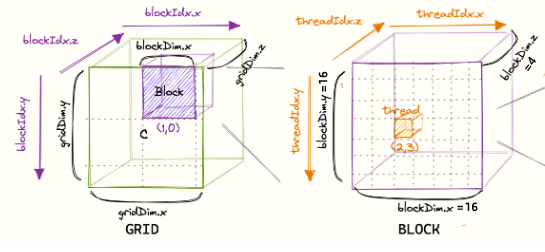
\includegraphics[width=0.5\textwidth]{assets/grid_block.png}
    \caption{Grid and Block Dimensions 3D division [1]}
    \label{fig:3}
\end{figure}
After defining the suitable block dimensions as (16, 16, 4), we move up and needed to compute the appropriate grid dimensions for the thread access to ensure that the entire 3D volume is accounted for. The grid dimensions are calculated by dividing the total number of rows/columns/depth by the corresponding block dimensions axis. However, since this division may not result in a whole number, the formula includes an adjustment to ensure full coverage of the data. Specifically, we add the block dimension minus one to the total size before performing integer division:

\begin{equation}
    \begin{aligned}
        \text{Grid dimension} &= \left\lceil \frac{\text{Total size}}{\text{Block size}} \right\rceil \\
        &\quad = \frac{\text{Total size} + \text{Block size} - 1}{\text{Block size}}
    \end{aligned}
\end{equation}
\\

So for our 3D grids and blocks, the grid dimensions for example the rows kernel become the following:
\begin{equation}
    \begin{aligned}
        \text{row\_grid} = \Bigg( 
        \left\lceil \frac{\text{rows} + \text{blockDim.x} - 1}{\text{blockDim.x}} \right\rceil, \\
        \left\lceil \frac{\text{cols} + \text{blockDim.y} - 1}{\text{blockDim.y}} \right\rceil, \\
        \left\lceil \frac{\text{depth} + \text{blockDim.z} - 1}{\text{blockDim.z}} \right\rceil
        \Bigg)
    \end{aligned}
\end{equation}

The kernel implementation identifies row, column, and depth indexes based on thread and block indexes, validating them to ensure bounds are respected. It then performs the 1D DWT along the respective dimension and stores results in a flattened row-major order. Two float pointers for input and temporary output data are used in device memory.\\

In the `dwt 3d` function, these pointers are swapped after each kernel to handle data dependencies. A mapping kernel then reorders the transformed volume back to its original layout. This mapping function, initially intended for multi-level DWT, ensures accurate data reordering. After completion, the temporary volume is freed, and the final data is returned to the host.

\section{Effective Use Of Advanced Facilities}

This section discusses the optimization methods implemented using CUDA facilities, with a focus on memory hierarchy. After loading the volume from the binary file, necessary data for kernel execution is ported to the device via the `toGPU` function.\\

Two main types of memory are transferred: the 3D volume and the filter low and high coefficients. The coefficients are hard-coded as 2D vectors in `assignment.cu`, with the db number determining the appropriate coefficient vector. These coefficients, essential for convolution, are transferred to device memory using either shared memory or constant memory.\\

For shared memory, additional float pointers are created for the coefficients alongside the volume pointer. In `toGPU`, the coefficients are fetched based on the db number, allocated using `cudaMalloc`, and copied to global memory with `cudaMemcpy`. Within the kernels, shared memory is defined locally, enabling threads within the same block to access it more quickly than global memory.\\

For constant memory, the coefficients are declared as constant memory in the kernel file. In `toGPU`, no memory allocation is required; instead, `cudaMemcpyToSymbol` copies the coefficients to constant memory. This memory is read-only, cached on the device, and allows kernels to access it faster than global memory.\\

Both implementations were analyzed using the NVIDIA profiler, focusing on data transfer times and kernel performance. It was noted that during profiling, CUDA initialization timings obscured the initial `cudaMalloc` and `cudaMemcpyToSymbol` timings.

\begin{figure}[h]
    \centering
    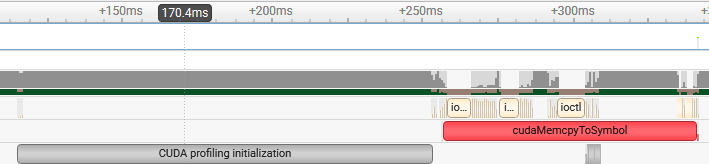
\includegraphics[width=0.5\textwidth]{assets/blamed-mem.png}
    \caption{cudaMemcpyToSymbol blamed for initalization time}
    \label{fig:4}
\end{figure}

\begin{figure}[h]
    \centering
    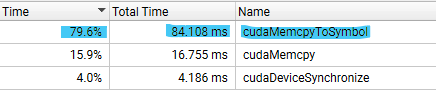
\includegraphics[width=0.5\textwidth]{assets/blamed-mem-sum.png}
    \caption{Summary showing abnormally high cudaMemcpyToSymbol time}
    \label{fig:5}
\end{figure}

Since the initial CUDA calls were responsible for initialization, the profiler attributed their timings to initialization overhead. To address this, additional `cudaEvent` markers were added to measure the memory transfer time. These events also reflected initialization timings, but they allowed for isolating the actual time taken for memory transfers after initialization.

\begin{figure}[h]
    \centering
    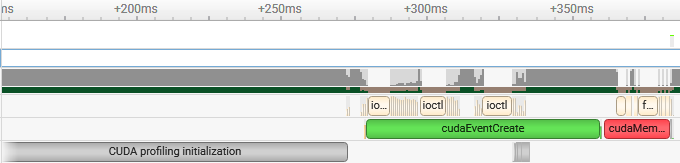
\includegraphics[width=0.5\textwidth]{assets/blamed-event.png}
    \caption{cudaEvent blamed for initalization time}
    \label{fig:6}
\end{figure}

\begin{figure}[h]
    \centering
    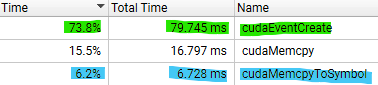
\includegraphics[width=0.5\textwidth]{assets/blamed-event-sum.png}
    \caption{Summary showing blamed time moved to cudaEvent}
    \label{fig:7}
\end{figure}

Since the blaiming issue is resolved and we know why our results initially seemed to be obscured by so much we can foucs back on the comparision between shared memory and constant memory. Each case will be analysed with the NVIDIA profiler and confiremd with a cudaEvent record of the time taken for the both the memory transfer and the kernel execution.

\begin{figure}[h]
    \centering
    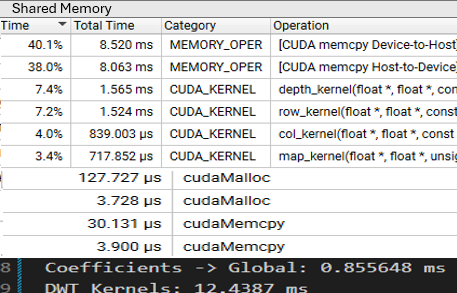
\includegraphics[width=0.5\textwidth]{assets/shared-prof.png}
    \caption{Shared Memory Profiling Results}
    \label{fig:8}
\end{figure}

\begin{figure}[h]
    \centering
    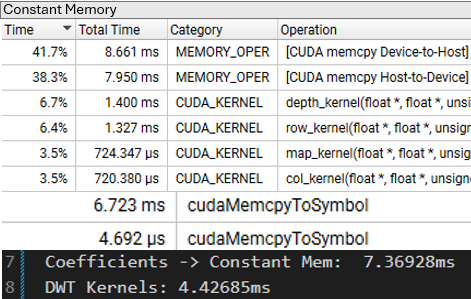
\includegraphics[width=0.5\textwidth]{assets/const-prof.png}
    \caption{Constant Memory Profiling Results}
    \label{fig:9}
\end{figure}

Figures 6 and 7 confirm results consistent with theoretical expectations. The shared memory implementation exhibits minimal data transfer time to device memory (0.856 ms) because of the small size of the coefficients. However, kernel execution is slower as shared memory is only accessible to threads within the same block, requiring each block to replicate the shared memory. In contrast, the constant memory implementation has a higher coefficient transfer time (7.369 ms) but benefits from device-wide access and caching, adding no overhead to kernel execution. Profiler results show that the constant memory implementation is faster and more efficient in this case due to reduced kernel overheads.

\begin{itemize}
    \item \textbf{Shared Memory Time:} Data Transfer Time + Kernel Execution Time = 0.856 ms + 12.439 ms = 13.295 ms
    \item \textbf{Constant Memory Time:} Data Transfer Time + Kernel Execution Time = 7.369 ms + 4.427 ms = 11.796 ms
    \item \textbf{Speed Up:} $\frac{\text{Total Shared Memory Time}}{\text{Total Constant Memory Time}} = \frac{13.295}{11.796} = 1.127$
\end{itemize}

To transfer the 3D volume to device memory, it must first be flattened into a 1D vector using row-major order. This is handled within the `toGPU` function. The row-major indexing follows the formula:  
\begin{equation}
    \text{index} = \text{depth} \times \text{rows} \times \text{cols} + \text{row} \times \text{cols} + \text{col}
\end{equation}  
This indexing ensures correct mapping by iterating through columns within rows at each depth, then progressing through rows at a depth, and finally across the depths of the volume. Once flattened, the volume is allocated and copied to device memory using `cudaMalloc` and `cudaMemcpy`, ensuring seamless access by the threads in the kernel. It is to be noted that the volume allocation could not be done in a more efficient manner such as using streams and concurrently executed memory transfers due to the nature of the data dependencies and the need for the entire volume to be available for the kernel execution.\\

After all kernel calls and the transformed volume has been mapped back to its original pointer, the data must be retrieved from device memory to the host. This is handled by the `toCPU` function, which allocates memory on the host and copies the flattened volume back using `cudaMemcpy`. The volume is then reshaped into its original 3D layout using the inverse of the row-major indexing formula, ensuring the data is correctly ordered for subsequent processing or visualization.\\

Further analysis of the constant memory implementation revealed an important optimization opportunity. By merging the two sets of constant coefficients for the low-pass and high-pass filters into a single constant memory array, the number of cudaMemcpyToSymbol calls was reduced to one. This change decreased memory transfer time and slightly improved performance. The kernel access logic was updated accordingly, using the coefficient length to determine the starting index of the high-pass coefficients in the array.

\begin{figure}[h]
\centering
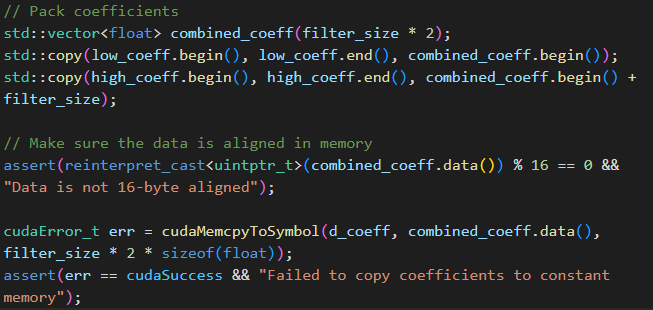
\includegraphics[width=0.5\textwidth]{assets/packed-coeffs.png}
\caption{Implementation of packed coefficients in a single array}
\label{fig:10}
\end{figure}

Finally, the use of size t variables instead of int is recommended for CUDA development. As a 64-bit unsigned integer type, size t aligns better with device memory and improves efficiency when indexing memory locations.

\section{Profile‐guided optimization:}
The NVIDIA profiler was previously utilized to analyze memory transfer and kernel execution times. To ensure accurate profiler results and reflect true implementation performance, all print statements and timing operations, such as cudaEvent markers, were wrapped in debug configurations. This eliminated interference from non-essential operations, resulting in more reliable profiler data.

\begin{figure}[h]
    \centering
    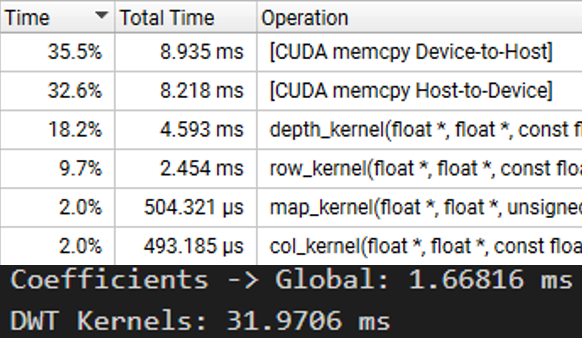
\includegraphics[width=0.5\textwidth]{assets/unoptim-sum.png}
    \caption{Profiler Summary of Unoptimized Code}
    \label{fig:11}
\end{figure}

One major shortcoming of the unoptimized code was the high memory access latency, as threads individually accessed global memory for the coefficients. This inefficiency significantly contributed to the high kernel execution times. The profiler summary in Figure 9 highlights this issue, showing that total kernel execution times dominated the performance profile.

\begin{figure}[h] 
    \centering 
    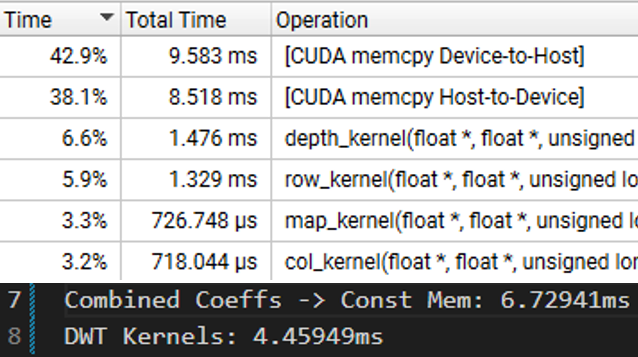
\includegraphics[width=0.5\textwidth]{assets/optim-sum.png} 
    \caption{Profiler Summary of Optimized Code} 
    \label{fig:12} 
\end{figure}

The final profiler results demonstrate substantial improvements over the unoptimized version. By leveraging constant memory, we introduced a minor overhead during the memory copy to symbols. However, this was outweighed by a significant reduction in kernel execution times, resulting in a marked decrease in the total execution time.

\section{Computation of speedup}

This section evaluates the speedup from parallelization by comparing the timing results of the serial and parallel implementations. A subset of the CHAOS dataset was preprocessed in Python, creating a smaller version with one-fourth the dimensions of the large dataset: \(512 \times 512 \times 78\) for the large, and \(128 \times 128 \times 20\) for the smaller dataset.

\begin{figure}[h]
    \centering
    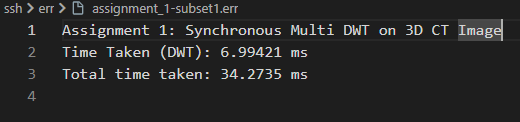
\includegraphics[width=0.5\textwidth]{assets/1-subset.png}
    \caption{Timing results for reference implementation (small set)}
    \label{fig:13}
\end{figure}

\begin{figure}[h]
    \centering
    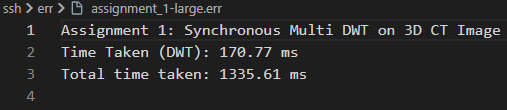
\includegraphics[width=0.5\textwidth]{assets/1-large.png}
    \caption{Timing results for reference implementation (large set)}
    \label{fig:14}
\end{figure}

The small dataset executes faster than the large one due to fewer iterations in the serial implementation. While the parallel implementation follows a similar trend, the difference might be less pronounced, as it benefits more from optimized block execution than reduced iterations.

\begin{figure}[h]
    \centering
    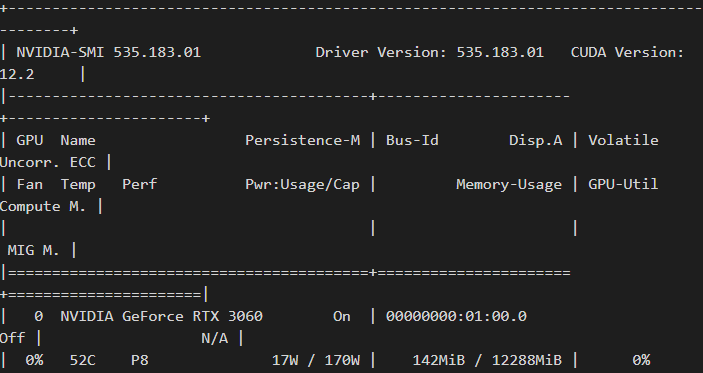
\includegraphics[width=0.5\textwidth]{assets/correct-device.png}
    \caption{Appropriate selection of device for parallel results}
    \label{fig:15}
\end{figure}

The snippet in Figure 13 shows that the appropriate device is being selected as '.sh' file includes 'nvidia-smi' to output the device information. This ensures that the parallel results are being executed on the correct device as stated in the requirements.

\begin{figure}[h]
    \centering
    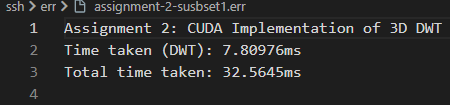
\includegraphics[width=0.5\textwidth]{assets/2-subset.png}
    \caption{Timing results for parallel implementation (small set)}
    \label{fig:16}
\end{figure}

\begin{figure}[h]
    \centering
    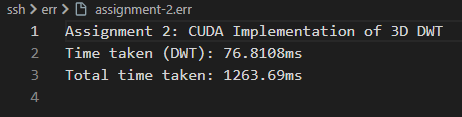
\includegraphics[width=0.5\textwidth]{assets/2-large.png}
    \caption{Timing results for parallel implementation (large set)}
    \label{fig:17}
\end{figure}

The parallel implementation shows a significant speedup over the serial implementation. The actual comparision will be done in the following section where it will be compared with the theoretical speedup acievable.

\section{Comparison Of Actual and Potential Speedup}

To estimate the theoretically available speedup, we use Amdahl's Law:
\begin{equation}
    S = \frac{1}{(1 - P) + \frac{P}{N}}
\end{equation}
Where:
\begin{itemize}
    \item $S$ is the theoretical speedup.
    \item $P$ is the proportion of the code that is parallelizable.
    \item $N$ is the number of cores available.
\end{itemize}
\noindent
Using the following hardware analysis:
\begin{verbatim}
NVIDIA-SMI 535.183.01
Driver Version: 535.183.01
CUDA Version: 12.2

GPU: NVIDIA GeForce RTX 3060
CUDA Cores: 3584 (approx)
Memory: 12GB
\end{verbatim}
\noindent
The RTX 3060 has approximately $N = 3584$ CUDA cores. Let us assume that the parallelizable portion of the code which is mainly composed of the 1D DWT operations is $P = 0.8$ (80\%).
Using Amdahl's Law:
\begin{equation}
    S = \frac{1}{(1 - 0.8) + \frac{0.8}{3584}} = 4.994
\end{equation}

Thus, the theoretical speedup with full parallelization and utilization of all available CUDA cores is approximately $S \approx 5.0$. Assuming that 80\% of the kernel is parallelizable and the overhead for memory transfers is negligible, the parallel implementation can achieve a 5x improvement over the serial implementation.\\

However, this theoretical speedup represents an idealized scenario and does not account for the task division and other practical factors. Kernel execution times depend heavily on data volume, thread count, block size, and data access patterns. Additionally, the data dependencies precent pose a limitation to full parallelization and speedup.\\

Furthermore, the for parallelization using CUDA, the memory bandwidth is a critical factor that can limit the speedup. The memory bandwidth must be contantly fed with data to keep the CUDA cores busy. But can be a bottleneck if the data transfer rate is slower than the processing rate of the CUDA cores.\\

The actual speedup achieved in the parallel implementation is calculated as:
\begin{equation}
    \text{Speedup (large)} = \frac{\text{Serial Time}}{\text{Parallel Time}} = \frac{170.77}{76.81} = 2.223
\end{equation}  

\begin{equation}
    \text{Speedup (small)} = \frac{\text{Serial Time}}{\text{Parallel Time}} = \frac{6.99}{7.81} = 0.895
\end{equation}

These results show that the theoretical speedup calculated using Amdahl's Law was significantly overestimated. Additionally, the actual speedup is lower, and for the small dataset, there is a slowdown due to memory transfer overhead. This indicates that the parallel implementation is only effective for large datasets, where the overhead is amortized over a greater number of iterations.

\section{Discussion of difficulties}
The primary challenge during parallelization was memory management and handling data dependencies. Flattening the volume, ensuring correct row-major indexing, and accessing the correct data for each thread proved complex. Additionally, managing synchronization and swapping of input and output pointers to process data accurately was initially challenging since the proper management of volume access with the thread and dimension indexing was not being properly assigned.\\

A major challenge that shifted the assignment's scope was implementing a multi-level DWT. Managing subbands and passing them between levels proved too complex within the time constraints. As a result, the focus shifted to a single-level DWT, enabling a more concentrated effort on parallelization and optimization. Future work could revisit multi-level DWT with more time for development.

\begin{thebibliography}{1}

    \bibitem{Siboehm2022}
    Siboehm, "CUDA Matrix-Matrix Multiplication (MMM)," 2022. [Online]. Available: \url{https://siboehm.com/articles/22/CUDA-MMM}. [Accessed: 17-Jan-2025].

    \bibitem{Copilot2024}
    GitHub Copilot, "Aided in C++, Python and Latex syntax coding," 2024. [Online]. Available: \url{https://github.com/features/copilot}. [Accessed: 2024].

\end{thebibliography}
\end{document}